\documentclass[11pt,letterpaper]{article}
\usepackage[spanish]{babel}
%\usepackage[ansinew]{inputenc}
\usepackage[utf8]{inputenc}
%\usepackage[latin1]{inputenc}
\usepackage[letterpaper,includeheadfoot, top=0.5cm, bottom=3.0cm, right=2.0cm, left=2.0cm]{geometry}
\renewcommand{\familydefault}{\sfdefault}

\usepackage{graphicx}
\usepackage{color}
\usepackage{hyperref}
\usepackage{amssymb}
\usepackage{url}
\usepackage{fancyhdr}
\usepackage{hyperref}
\usepackage{subfig}
\usepackage{acronym} %Acronimos

\usepackage{listings} %Codigo
\lstset{language=C, tabsize=4,framexleftmargin=5mm,breaklines=true}

% -------------------------ACRONIMOS --------------------------------------------
\acrodef{RAM}{\textit{Random Access Memory}}
\acrodef{RISC}{\textit{Reduced Instruction Set Computing}}
\acrodef{ALU}{\textit{Arithmetic Logic Unit}}
\acrodef{EULA}{\textit{End-User License Agreement}}
\acrodef{GPL}{\textit{General Public License}}
\acrodef{RTOS}{\textit{Real Time Operating System}}

\begin{document}
% --------------- ---------PORTADA --------------------------------------------
\newpage
\pagestyle{fancy}
\fancyhf{}
%-------------------- CABECERA ---------------------
\fancyhead[L]{ 
\includegraphics[scale=0.9]{img/logo_die.pdf} }
%------------------ TÍTULO -----------------------
\vspace*{6cm}
\begin{center}
\Huge  {Avance Capitulo 2} \\
\vspace{1cm}
\LARGE {EL6908 - Introducción al Trabajo de Título}\\
\vspace{0.5cm}
\LARGE {\textit{Diseño e Implementación de una plataforma para experimentos en microgravedad y de electrónica en ambiente hostil con Nano-Sat\'elites}}\\
\end{center}
%----------------- NOMBRES ------------------------
\vfill
\begin{flushright}
\begin{tabular}{ll}
\textbf{Autor} &: Jos\'e Ogalde O.\\
\textbf{Profesor Guía} &: Marcos Díaz Q.\\
\textbf{Profesor EL6908} &: Jorge Lopez H.\\
& \today\\
& Santiago, Chile.
\end{tabular}
\end{flushright}

% ·············· ENCABEZADO ············
\newpage
\pagestyle{fancy}
\fancyhf{}
%\fancyhead[L]{\rightmark}
\fancyhead[L]{\small \rm \textit{Sección \rightmark}}
\fancyhead[R]{\small \rm \textbf{\thepage}}
\fancyfoot[L]{\small \rm \textit{Avance Capítulo 2}}
\fancyfoot[R]{\small \rm \textit{EL6908 - Introducción al Trabajo de Título}}
%\fancyfoot[C]{\thepage}
\renewcommand{\sectionmark}[1]{\markright{\thesection.\ #1}}
\renewcommand{\headrulewidth}{0.5pt}
\renewcommand{\footrulewidth}{0.5pt}

% =============== INDICE ===============

\tableofcontents
\listoffigures
\listoftables

% =============== CUERPO ===============
\newpage

\section{Antecedentes Teóricos}

En el presente informe se entrega un avance del Capitulo 2 del trabajo de título del autor. El objetivo es desarrollar el marco teórico más importantes involucrados en este trabajo de título.

% ============= SISTEMAS EMBEBIDOS ==============
\subsection{Sistemas embebidos}
Los computadores personales son utilizados por gran parte de la población dado que se caracterizan por tener capacidad para atender una cantidad importante de procesos dispuestos por un sistema operativo en orden para atender diferentes aplicaciones  del usuario final. Un microcontrolador tambi\'en es un tipo de computador salvo que sus recursos normalmente son más limitados que los de un computador personal. Además, un microcontrolador normalmente tiene más flexibilidad para el uso directo de perif\'ericos y poder comunicarse a nivel de máquina con otro dispositivo electrónico.

Un sistema embebido está compuesto por uno más microcontroladores en conjunto con dispositivos electrónicos con los cuales comunicarse para realizar alguna tarea. 
El hardware que compone a un microcontrolador está fija por lo que el desarrollador de sistemas embebidos solamente tiene acceso a la programación de \'este en conjunto con la correcta interconexión con otros dispositivos electrónicos. Debe considerarse que a diferencia de un computador personal, el programa que provee la funcionalidad del microcontrolador se denomina \textit{firmware}, ya que en general es específico para la plataforma de hardware utilizada.

\subsubsection{Microcontroladores PIC}
Este trabajo se concentra en el uso de los microcontroladores PIC desarrollados por la compañía Microchip como cerebro de la plataforma. La familia de microcontroladores  PIC es bastante amplia adaptándose a un amplio rango de necesidades, la tabla \ref{pic_list} resume las principales características de los diferentes modelos y puede ser utilizada como una guía para determinar el dispositivo adecuado según la aplicación:

% ················ TALBA ·················
\begin{table}[ht!]
\caption{Resumen de familias de Microchip}\label{pic_list}
\centering 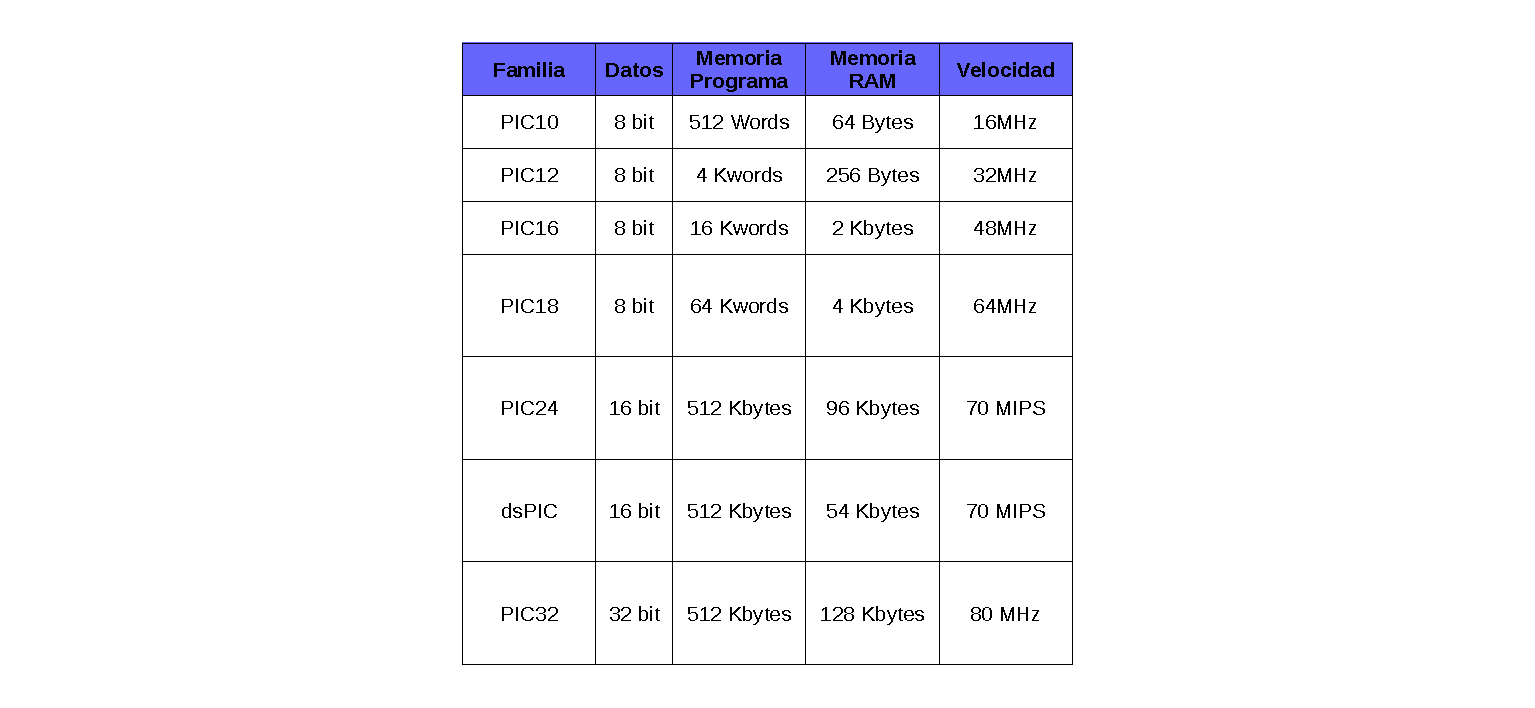
\includegraphics[width=\textwidth]{img/pic_list.pdf}
\end{table}
%··········································
\subsection{Microcontrolador}
Un microcontrolador es un computador pequeño dentro de un solo circuito integrado, que posee un solo nucelo de proceso, memoria y perif\'ericos de entrada/salida. Los microcontroladores estan diseñados para los sistemas embebidos, en contraste a los microprocesadores utilizados en computadores personales u otras aplicaciones de propósito general.

Los microcontroladores son utilizados en dispositivos y productos automáticamente controlados como por ejemplo, controles remotos, sistema de control de automóviles, etc.

\subsection{Nano-Sat\'elites}
Corresponden a los sat\'elites artificiales con una masa entre 1 y 10 kg. Con los continuos avances en la minaturización y capacidad de la electrónica en conjunto al uso de constelaciones de sat\'elites, los nano-sat\'elites están crecientemente capaces de desempeñarse bien en misiones comerciales. Un caso destacable son los nano-sat\'elites que siguen el protocolo CubeSat, cuyo primer lanzamiento fue el 2003 y en el año 2012 se lanzaron 75 sat\'elites al espacio.

\subsubsection{CubeSat}
Es un tipo de nano-sat\'elite hecho de multiples unidades cúbicas de 10x10x10 cm, no tiene más de 1.3 kg de masa por unidad y a menudo utiliza componentes \textit{commercial off-the-shelf} (COTS) para su electrónica y estructura.

Los usos típicos involucran experimentos que pueden ser miniaturizados o experimentos para servir a propósitos como la observación del planeta o comunicación de radio amateur.

Uno de los atractivos de los CubeSats es su bajo costo en comparación a otras tecnologías satelitales. Esto lo convierte en buen candidato para probar nuevas tecnologías a bordo de estas plataformas dado que su costo puede justificar misiones riesgosas.

\subsubsection{Proyecto SUCHAI}
  \textit{Satellite of the University of CHile for Aerospace Investigation} (SUCHAI) corresponde al primer sat\'elite artificial diseñado y desarrollado localmente en Chile por un conjunto de estudiantes de pregrado y profesores del Departamento de Ingeniería Elctrica de la Universidad de Chile.
SUCHAI es un nano-sat\'elite de tipo CubeSat de una unidad (aproximadamente 1 kg), cuyo objetivo principal es educacional y científico.
La misión de SUCHAI se considera en los siguientes \textit{payloads}
\begin{itemize}
\item \textbf{Langmuir probe: } Estudio de la ionósfera en sincronización con el \textit{incoherent scatter radar} (ISR) tomando medidas simultáneas de la variación en la densidad de electrones en la ionósfera.
\item \textbf{Eletrónica fuera del equilibrio: } Un circuito RC para estudiar las fluctuaciones fuera de equilibrio en la potencia inyectada al estar en un ambiente hostil como el espacio.
\item \textbf{Experimento termal: } Estudia la disipación de calor en dispositivos electrónicos en un ambiente vacío.
\item \textbf{Cámara: } Una cámara digital para analizar la factibilidad de observar la tierra desde un cubesat.
\item \textbf{Receptor GPS: } Un módulo receptor GPS para obtener la posición del sat\'elite y aprender cómo utilizarlo en futuras misiones.
\end{itemize}

\subsubsection{Payload}
\subsection{Bus}
\subsubsection{PC-104}
\subsection{Actuadores y Sensores}
\subsubsection{Conversor ADC}
\subsubsection{Conversor DAC}
\subsection{Controlador de hardware}
\subsection{Microgravedad}
\subsection{Sistema fuera de equilibrio}
\subsection{Circuito pasivo}
\subsubsection{Circuito RC}
\subsubsection{Potencia inyectada}
\end{document}
